\chapter{Faste stoffer}
De fleste faste stoffer er bygget opp av atomer plassert i en periodisk krystallstruktur. Detaljene i denne strukturen er avgjørende for egenskapene til materialet, og vi skal se på noen slike egenskaper her. Det finnes også noen faste stoffer som ikke har en slik periodisk krystallstruktur, f.eks. glass der atomene har tilfeldige plasseringer. Biologiske materialer som tre har en mer komplisert struktur. I dette avsnittet begrenser vi oss til å se på materialer med en fast krystallstruktur.

Når vi skal se på egenskapene til faste stoffer må vi skille mellom isolatorer og ledere/metaller.\footnote{I tillegg har vi også halvledere som har mest til felles med isolatorer, men som likevel har en del interessante egenskaper vi ikke ser hos isolatorene. Dette blir imidlertid ikke diskutert her.} I et metall er noen av elektronene så løst bundet at de essensielt sett kan bevege seg fritt i hele metallstykket. Det er dette som gjør at metaller kan lede elektrisk strøm, og det gjør også at elektronene kan gi et viktig bidrag til metallets varmeledningsevne. I isolatorer derimot er alle elektronene tett bundet til atomkjernene. Dermed kan ikke elektronene bidra til transport av verken elektrisk strøm eller varme slik som i metaller, og de termiske egenskapene bestemmes utelukkende av hvordan atomene i krystallstrukturen vibrerer.

\section{Termisk utvidelse}
Tilnærmet alle\footnote{Et viktig unntak her er vann i temperaturområdet 0 til $4^\circ~\mathrm{C}$.} materialer utvider seg når de varmes opp og trekker seg sammen når de kjøles ned. Vi kan  utvidelsen av et krystalinsk stoff kvalitativt ved å se på atomenes mikroskopiske bevegelse. Vi modellerer krystallen som en samling av punktmasser som er holdt på plass av et nettverk av fjærer mellom dem, se figur \ref{fig:fastelegemer:krystall}. Punktmassene representerer atomene, mens fjærene representerer de elektriske kreftene som virker mellom dem. 

Vi innser at denne konfigurasjonen gir en likevektsposisjon for hvert enkelt atom der summen av krefter som virker på det er lik 0. Hvis atomet flyttes litt bort fra likevektsposisjonen vil det virke krefter på det som trekker det mot likevektsposisjonen. Hvis vi antar at kreftene mellom atomene oppfører seg som ideelle fjærer gir disse kreftene opphav til et harmonisk potensial som vist i figur \ref{fig:fastelegemer:harmonisk}. Så lenge atomet har energi $> 0$ vil det vibrere om likevektsposisjonen sin med en amplitude som er avhengig av hvor stor energi\footnote{Kvantemekanikken forteller oss at atomet aldri kan ha 0 energi, og at energien bare kan være en av et diskret sett verdier. Dette er ikke viktig for denne diskusjonen, så vi ser ikke mer på det her.} det har---og derfor avhengig av temperaturen. 

I denne modellen ser vi at når temperaturen øker vil atomene kunne bevege seg lengre vekk fra likevektspunktet sitt, men den gjennomsnittlige avstanden mellom atomene forblir den samme. Dette ville ikke gi noen målbar termisk utvidelse, så denne modellen er opplagt ikke riktig. Der modellen feiler er at den modellere potensialet atomet beveger seg i som symmetrisk om likevektsposisjonen. Figur \ref{fig:fastelegemer:LennardJones} viser hvordan den potensielle energien, $U(r)$, avhenger av avstanden til naboatomene, $r$, i en typisk krystall. Av kvantemekaniske årsaker er det kun et diskret sett av energitilstander atomet kan befinne seg i. Ved svært lave temperaturer vil praktisk talt alle atomene i krystallen være i den laveste energitilstanden, $E_0$. Når temperaturen øker vil en del atomer eksiteres opp til høyere energitilstander. Vi ser fra potensialgrafen at da skjer to ting: For det første øker rekkevidden av $r$-verdier atomet kan ha. Det vil si at vibrasjonsamplituden øker. For det andre---og viktigere for vår diskusjon---når atomene går opp til høyere energitilstander øker den gjennomsnittlige avstanden mellom atomene og det er dette som forklarer den termiske utvidelsen.

\begin{figure}[tp]
	\begin{center}
	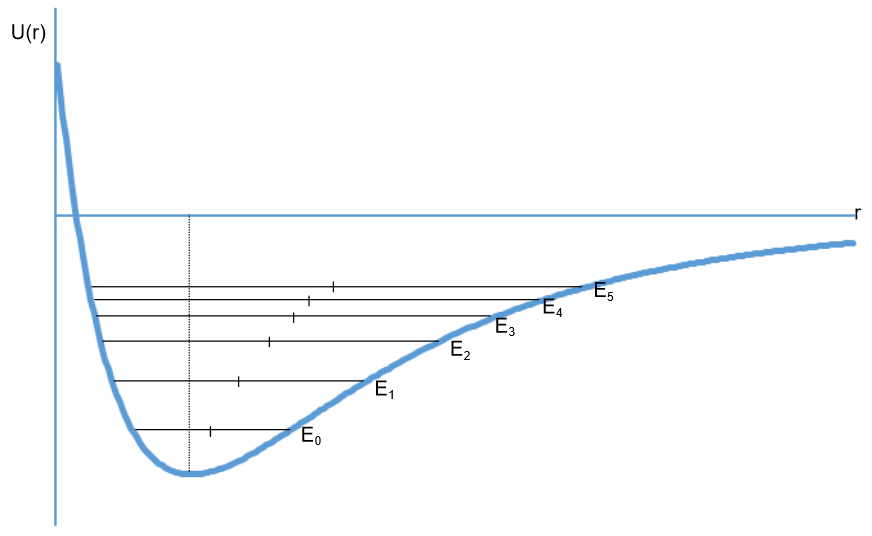
\includegraphics[width=.8\textwidth]{./LennardJones}
	\end{center}
	\caption{Figuren viser et typisk potensial for et atom i en krystall. Av kvantemekaniske årsaker er det kun et diskret sett av energitilstander atomet kan være i. De seks laveste er merket av på figuren som $E_0, E_1, \ldots$. Gjennomsnittlig avstand $r$ til naboatomene er også merket av for hver av de seks energitilstandene.}
	\label{fig:fastelegemer:LennardJones}
\end{figure}

\subsection{Lineær utvidelse}
Makroskopisk viser det seg at termisk utvidelse beskrives godt som direkte proporsjonal med temperaturen. Hvis vi har en stav som ved temperatur $T_0$ har lengde $L_0$ vil den da ved temperatur $T+\Delta T$ ha lengde $L+\Delta L$ der
\begin{equation}
	\Delta L = \alpha L_0\Delta T.
	\label{eq:fastelegemer:deltaL}
\end{equation}
Her er $\alpha$ en koeffisient som er spesifikk for det materialet vi jobber med. Vi ser av ligning (\ref{eq:fastelegemer:deltaL}) at $\alpha$ må ha enhet $\mathrm{K}^{-1}$ (eller $\mathrm{^\circ C}^{-1}$). Typiske verdier av koeffisienten $\alpha$ er av størrelsesorden $10^{-5}~\mathrm{K}^{-1}$.

\subsection{Volumutvidelse}
I tråd med den lineære utvidelsen vi nettopp har sett på vil naturlig nok også volumet av objekter øke når temperaturen øker. Vi skal nå se på volumøkningen av en kube med sidekanter $L_0$. Vi vet at hver sidekant øker lengden fra $L_0$ til $L = L_0+\Delta L$. Dette betyr at volumet øker fra $V_0 = L_0^3$ til $V = (L_0+\Delta L)^3$. Når vi setter inn 	(\label{eq:fastelegemer:deltaL}) finner vi
\begin{displaymath}
\begin{aligned}
	V &= \left[ L_0 + \alpha L_0 \Delta T\right]^3 \\
	&=L_0^3\left[1+\alpha \Delta T\right]^3 \\
	&=V_0 \left[1 + 3\alpha\Delta T + 3(\alpha\Delta T)^2 + (\alpha\Delta T)^3 \right]
\end{aligned}
\end{displaymath}
Siden den termiske utvidelsen for de fleste materialer er svært liten er $\alpha\Delta T\ll1$ for alle realistiske verdier av $\Delta T$. Det betyr at leddene med $(\alpha\Delta T)^2$ og $(\alpha\Delta T)^3$ er av neglisjerbar betydning og vi kan med god presisjon si at 
\begin{displaymath}
	V = V_0(1+3\alpha\Delta T).
\end{displaymath}
Vi ser altså at også den termiske volumutvidelsen til en god tilnærming er direkte proporsjonal med temperaturforskjellen: $V = V_0 + \Delta V$ med
\begin{equation}
	\Delta V = \beta V_0 \Delta T,
\end{equation}
der $\beta = 3\alpha$ er volumutvidelseskoeffisienten.

\section{Varmekapasitet}

\section{Varmeledning}